	\begin{center}
		\section{动态规划（dp）}
	\end{center}

	\begin{multicols*}{2}

		\subsection{二进制子集枚举技巧}
		如果要枚举 $n$ 个元素的所有子集，最直接的写法是把每个集合看成一个二进制数，范围就是 $[0, 2^n - 1]$。

		\begin{minted}{cpp}
for (int s = 0; s < (1 << n); s++) {
	// s 的二进制表示对应一个子集
}
		\end{minted}

		\subsubsection{枚举某个集合的所有子集}
		如果已经有一个集合 \texttt{mask}，想要只枚举它的所有子集，常用下面这个写法。

		\begin{minted}{cpp}
for (int sub = mask; sub; sub = (sub - 1) & mask) {
	// sub 是 mask 的一个非空子集
}
		\end{minted}

		它的原理是，\texttt{sub - 1} 会把 \texttt{sub} 最低位的一个 $1$ 变成 $0$，并把它右边的若干位全部变成 $1$。随后再与 \texttt{mask} 做一次按位与，就会把不属于 \texttt{mask} 的位置全部清掉，于是得到一个更小但仍然合法的子集。

		因此，这个过程会按照从大到小的顺序，不重不漏地枚举出 \texttt{mask} 的所有非空子集。

		如果还需要处理空集，可以写成下面这样。注意 \texttt{sub == 0} 时必须及时跳出，不然会死循环。

		\begin{minted}{cpp}
for (int sub = mask;; sub = (sub - 1) & mask) {
	// sub 是 mask 的一个子集，包含空集
	if (sub == 0) {
		break;
	}
}
		\end{minted}

		这个技巧在状压 DP 中非常常见。若外层再枚举所有 \texttt{mask}，内层枚举它的全部子集，总复杂度是 $O(3^n)$。

		\subsubsection{枚举固定大小的子集}
		如果只关心恰好选了 \texttt{use} 个元素的状态，就没必要把所有状态都扫一遍再用 \texttt{popcount} 过滤。可以直接枚举二进制中恰好有 \texttt{use} 个 $1$ 的状态。

		\begin{minted}{cpp}
for (int use = 0; use <= K; ++use) {
	long long sta = (1LL << use) - 1;
	while (sta < (1LL << K)) {
		// sta 的二进制中恰好有 use 个 1

		if (sta == 0) break;  // use=0 时只对应空集这一个状态，避免下面除零
		long long c = sta & -sta;
		long long r = sta + c;
		sta = (((r ^ sta) >> 2) / c) | r;
	}
}
		\end{minted}

		这里先令 \texttt{sta = (1LL << use) - 1}，也就是二进制下最小的、恰好含有 \texttt{use} 个 $1$ 的状态。后面的转移则负责直接跳到“下一个同样有 \texttt{use} 个 $1$ 的状态”。

		\texttt{c = sta \& -sta} 会取出最低位的 $1$，\texttt{r = sta + c} 可以理解为把最靠右、还能向左移动的一位 $1$ 往前推一格。这样一来，右侧结构会被打乱，再用最后那一行把剩余的若干个 $1$ 重新挪到最右边，于是就得到了下一个更大的合法状态。

		这个写法常被称为 \texttt{Gosper's hack}。它会按照从小到大的顺序，直接跳到下一个二进制中有相同个数 $1$ 的状态。若 \texttt{use = 0}，则只对应空集这一个状态。

		\subsubsection{枚举补集元素做前向转移（附「交判子集」）}

		状压 DP 常写成\textbf{前向（push）}形式：站在状态 \texttt{sta} 上，枚举一个\textbf{还没被选进来}的元素 \texttt{to}，把 \texttt{dp[sta]} 推给 \texttt{dp[sta | (1 << to)]}。这时不要写成「扫 $0 \ldots n-1$ 再用 \texttt{if} 过滤掉已在 \texttt{sta} 里的位」，而是直接把补集掏出来逐位剥：

		\begin{minted}[highlightlines={4,6}]{cpp}
int rem = full & (~sta);   // 还没选的元素集合
while (rem) {
	// 取出最低位的 1 所在下标
	int to = __builtin_ctz(rem);
	// 剥掉最低位的 1，进入下一轮
	rem &= rem - 1;
	// ... 用 to 做转移 ...
}
		\end{minted}

		两点好处：循环次数等于\textbf{补集大小}而不是 $n$（\texttt{sta} 越满越省，整层下来常数明显更小）；并且 \texttt{\_\_builtin\_ctz} 直接给出\textbf{下标}，省掉「先枚举下标再判位」的那次 \texttt{if}。注意 \texttt{full \& (\textasciitilde sta)} 的 \texttt{full} 掩码不能少，否则 \texttt{\textasciitilde sta} 的高位全是 $1$，\texttt{ctz} 会跑到 $n$ 以外的位上去。\texttt{\_\_builtin\_ctz} 只吃 \texttt{unsigned int}（$32$ 位），$64$ 位状态要用 \texttt{\_\_builtin\_ctzll}；另外 \texttt{ctz(0)} 是 UB，所以判空必须放在循环条件里。

		\textbf{用「交」判子集}：转移往往还带一个前置条件——元素 \texttt{to} 有一个\textbf{前驱依赖集合} \texttt{pre[to]}，只有依赖全部就位才能选它，即 $\texttt{pre[to]} \subseteq \texttt{sta}$。位掩码下的子集判定就是一次按位与：
		$$A \subseteq B \iff A \mathbin{\&} B = A \iff A \mathbin{\&} \sim\! B = 0 \iff A \mathbin{|} B = B$$

		\begin{center}
			\begin{tabular}{l|c|l}
				\hline
				含义 & 位串 & 说明 \\
				\hline
				\texttt{sta}          & \texttt{1 0 1 1} & 已选集合 \\
				\texttt{pre[to]}      & \texttt{0 0 1 1} & 依赖集合 \\
				\texttt{pre[to]\&sta} & \texttt{0 0 1 1} & $=$ \texttt{pre[to]}，可转移 \\
				\hline
				\texttt{pre[to]}      & \texttt{0 1 1 0} & 换一个依赖 \\
				\texttt{pre[to]\&sta} & \texttt{0 0 1 0} & $\neq$ \texttt{pre[to]}，不可转移 \\
				\hline
			\end{tabular}
		\end{center}

		合起来就是「有依赖约束的排列计数 / 拓扑序计数」的标准骨架：

		\begin{minted}[highlightlines={8}]{cpp}
// dp[sta] = 只用 sta 内元素、且满足依赖的合法前缀方案数
vector<uint32_t> dp(1 << n);
dp[0] = 1;
const int full = (1 << n) - 1;
for (int sta = 0; sta < full; ++sta) {
	if (!dp[sta]) continue;          // 剪掉不可达状态
	int rem = full & (~sta);
	while (rem) {
		int to = __builtin_ctz(rem);
		rem &= rem - 1;
		// pre[to] 全部就位才允许放 to
		if ((pre[to] & sta) == pre[to]) {
			dp[sta | (1 << to)] += dp[sta];
		}
	}
}
cout << dp[full] << "\n";
		\end{minted}

		复杂度 $O(2^n \cdot n)$。$n = 26$ 时 $2^{26} \cdot 26 \approx 1.7 \times 10^9$ 次极轻的位运算，配合 \texttt{if (!dp[sta]) continue} 的剪枝和 \texttt{uint32\_t}（自然溢出当作 $\bmod 2^{32}$，省掉取模）仍然能过——牛客多校 2026 第 6 场 Full Alphabet 即此模型，依赖集合由 Z 函数导出。

		\subsection{SOS DP（Sum / Max over Subsets，高维前缀和）}

		给定一个长度为 $2^N$ 的数组 $f[\,\cdot\,]$（下标看成 $N$ 位二进制掩码），希望对每个 $mask$ 求出
		$$F[mask] = \bigoplus_{sub \subseteq mask} f[sub]$$
		其中 $\bigoplus$ 可以是 $+$ / $\max$ / $\min$ / 异或等任何幺半群运算。直接枚举子集是 $O(3^N)$；SOS DP 通过\textbf{逐位扩展}把它压到 $O(N \cdot 2^N)$。

		核心思想是把每一位看成一个维度，依次做「沿第 $i$ 维的一维前缀」：当处理到第 $i$ 位时，若 $mask$ 第 $i$ 位是 $1$，就把 $mask$ 与 $mask \oplus (1 \!\ll\! i)$（去掉第 $i$ 位）合并。等价于沿 $N$ 个超立方体维度各做一遍一维前缀和。

		\textbf{对偶版}：超集而非子集，即 $F[mask] = \bigoplus_{mask \subseteq sup} f[sup]$。把转移方向反过来，把「有第 $i$ 位的从无第 $i$ 位的吸收」改成「无第 $i$ 位的从有第 $i$ 位的吸收」即可。

		\subsubsection{典型应用：按位无交最大值}

		问题：给定 $n$ 个非负整数 $a_1, \dots, a_n$，对每个 $i$ 找出最大的 $a_j$ 使得 $a_i \,\&\, a_j = 0$（按位无交集，二进制位上互不相交）。

		做法：
		\begin{itemize}
			\item 用 $dp[mask] = \max\{a_j : a_j \subseteq mask\}$（位掩码意义下的子集），初值 $dp[a_j] = a_j$。
			\item 跑一遍\textbf{子集 max}的 SOS DP，得到「掩码 $mask$ 下所有子集中最大的 $a_j$」。
			\item 对询问 $i$，答案 = $dp[\,\overline{a_i}\,]$，因为 $a_j$ 与 $a_i$ 按位无交 $\iff a_j \subseteq \overline{a_i}$。
		\end{itemize}

		复杂度 $O((V + n) \cdot \log V)$，其中 $V = \max a_i$。

		\begin{minted}{cpp}
void solve() {
	int n;
	cin >> n;
	vector<int> a(n);
	for (int &x : a) cin >> x;
	const int V = ranges::max(a);
	const int N = 32 - __builtin_clz(V); // 用到的位数
	vector<int> dp(1 << N);
	for (int x : a) dp[x] = x;           // 标记原始集合

	// SOS DP：dp[mask] = max{a_j : a_j 的位是 mask 的子集}
	for (int i = 0; i < N; i++) {
		for (int mask = (1 << N) - 1; mask >= 0; mask--) {
			if ((mask >> i) & 1) {
				dp[mask] = max(dp[mask],
				               dp[mask ^ (1 << i)]);
			}
		}
	}

	// 查询：与 a[i] 按位无交 等价于 是 ~a[i] 的子集
	for (int i = 0; i < n; i++) {
		int q = (~a[i]) & ((1 << N) - 1);
		cout << (dp[q] == 0 ? -1 : dp[q]) << " \n"[i == n - 1];
	}
}
		\end{minted}

		\textbf{要点}：
		\begin{itemize}
			\item 第二重循环\textbf{方向无关}（顺序、逆序都对），因为转移只涉及「同一 $i$ 位下，$mask$ 与去掉该位的 $mask \oplus (1 \!\ll\! i)$」，去掉位的 $mask$ 在本轮不会被本轮的更新二次覆盖（它的第 $i$ 位是 $0$，进不了 \texttt{if} 分支）。
			\item 用「0 表示未出现」的哨兵时，要确保 $a_j \neq 0$；否则要换 \texttt{-INF} 或者额外的 \texttt{exists} 标志位。
			\item 改成求\textbf{方案数}就把 \texttt{max} 换成 \texttt{+}，求\textbf{异或}就换成 \texttt{\^{}}，模板完全一致。
		\end{itemize}

		\subsection{子集格最短路（超集和 + 状压 DP 求最优排列）}

		\textbf{通用模型}：要给 $m$ 个元素定一个处理顺序（一个排列），把元素 $j$ 排在「已处理集合 $S$」之后的代价是 $\mathrm{cost}(S, j)$——注意它\textbf{只跟 $S$ 和 $j$ 有关}，跟 $S$ 内部的先后顺序无关。求总代价最小的排列。

		这类问题等价于\textbf{子集格上的最短路}：把 $2^m$ 个子集当结点，从 $S$ 向 $S \cup \{j\}$ 连一条权为 $\mathrm{cost}(S, j)$ 的边，答案就是 $\varnothing \to \{0,1,\dots,m-1\}$ 的最短路。因为边只从小集合指向大集合，图天然是 DAG，按 $mask$ 升序扫一遍就是拓扑序，不用 Dijkstra。

		\begin{center}
		\begin{tikzpicture}[scale=0.85, every node/.style={font=\scriptsize},
			st/.style={draw, rounded corners=2pt, inner sep=1.6pt, fill=white},
			ed/.style={-{Stealth[length=4pt]}, gray!60}]
			\node[st] (e)   at (0,0)      {$\varnothing$};
			\node[st] (a0)  at (-2.1,1.3) {$\{0\}$};
			\node[st] (a1)  at (0,1.3)    {$\{1\}$};
			\node[st] (a2)  at (2.1,1.3)  {$\{2\}$};
			\node[st] (b01) at (-2.1,2.6) {$\{0,1\}$};
			\node[st] (b02) at (0,2.6)    {$\{0,2\}$};
			\node[st] (b12) at (2.1,2.6)  {$\{1,2\}$};
			\node[st] (f)   at (0,3.9)    {$\{0,1,2\}$};
			\foreach \x/\y in {e/a0, e/a2, a0/b01, a0/b02, a1/b01, a2/b02, a2/b12, b01/f, b02/f}
				\draw[ed] (\x) -- (\y);
			% 一条候选顺序：先 1，再 2，最后 0
			\draw[-{Stealth[length=5pt]}, red!80!black, very thick] (e)   -- (a1)
				node[midway, left=1pt, red!70!black] {$\mathrm{cost}(\varnothing,1)$};
			\draw[-{Stealth[length=5pt]}, red!80!black, very thick] (a1)  -- (b12)
				node[midway, below right=0pt and 1pt, red!70!black] {$\mathrm{cost}(\{1\},2)$};
			\draw[-{Stealth[length=5pt]}, red!80!black, very thick] (b12) -- (f)
				node[midway, right=1pt, red!70!black] {$\mathrm{cost}(\{1,2\},0)$};
		\end{tikzpicture}
		\end{center}

		图中红色一条 $\varnothing \to \{1\} \to \{1,2\} \to \{0,1,2\}$ 对应排列 $(1, 2, 0)$，路径长度就是这个排列的总代价；$m!$ 种排列被压进 $2^m$ 个结点里，这正是状压 DP 省下阶乘的地方。

		\textbf{代价怎么来}：常见形态是「每条数据带一个能力掩码 $mask$ 与一组权 $w[\,\cdot\,]$，元素 $j$ 排在 $S$ 之后要付出所有 $mask \supseteq S$ 的那些数据的 $w[j]$」。先把每条数据按 $mask$ 装桶累加，再对每一维做\textbf{超集和}（上一节 SOS DP 的对偶版），桶就原地变成了 $\mathrm{cost}(S, j)$。

		\textcolor{red!75!black}{\textbf{SOS DP 的精髓：外层先枚举维度，内层才枚举状态}}。高维前缀和 / 超集和的本质是「\textbf{对每一维各做一次}一维前缀和」，$m$ 维就是 $m$ 轮，每轮把这一维「压平」。两层循环\textbf{写反就是错的}：外层若是状态、内层是维度，同一个状态在一次内层里连着吃多个方向的超集，而那些超集已被部分更新，导致\textbf{重复计数}。$m = 2$ 的反例（记初值 $f_{00}, f_{01}, f_{10}, f_{11}$，$S$ 倒序）：

		\begin{center}
			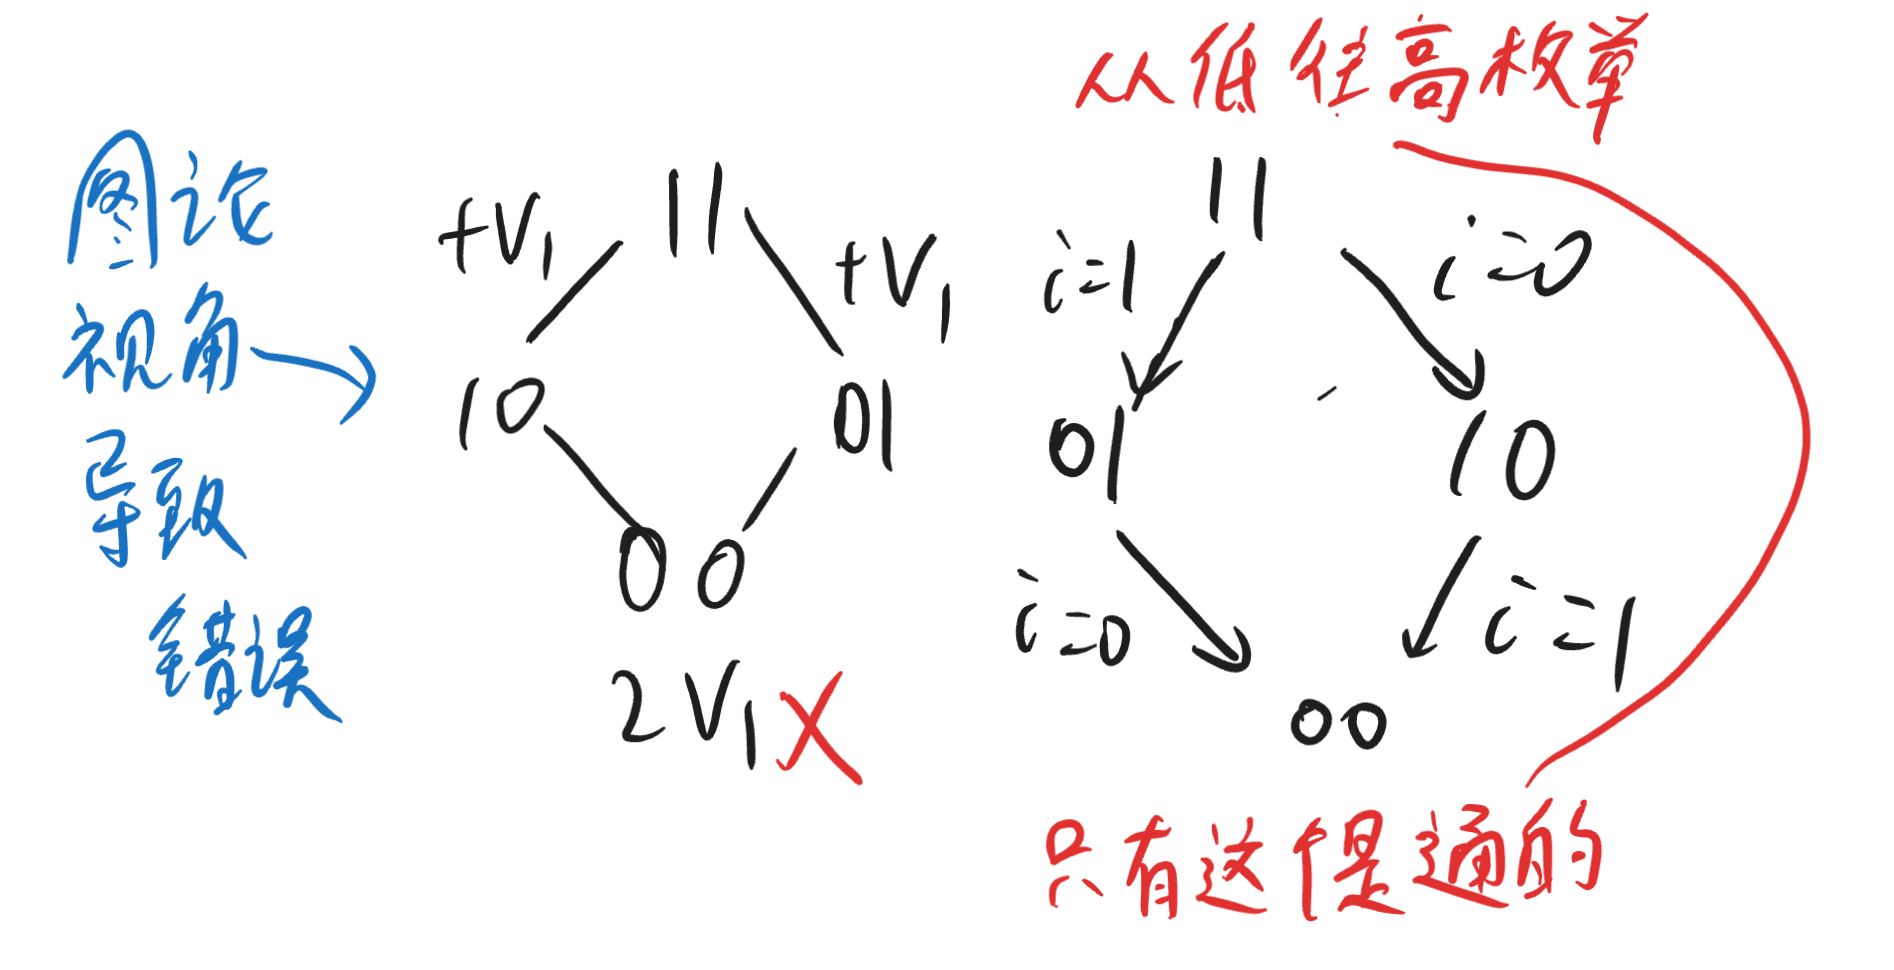
\includegraphics[width=\linewidth]{image/sos-dp-dimension-vs-graph-view.png}
		\end{center}

		\textbf{左半（错）}：按「图论最短路」的直觉去想，$11$ 沿两条边各把 $V_1$ 送给 $10$ 与 $01$，两路再汇到 $00$，于是 $00$ 吃进 $2V_1$——$f_{11}$ 被经 $10$ 与 $01$ 各加了一次。\textbf{右半（对）}：维度在外时每一轮只沿\textbf{一个}维度走，$11 \to 00$ 的两条边必然分属 $i = 1$ 与 $i = 0$ 两个不同轮次，所以 $11$ 只会被累加一次，「只有这条是通的」。

		反过来，维度在外时\textbf{内层状态的枚举顺序无所谓}（正序倒序都对）：本轮只改第 $i$ 位为 $0$ 的状态，而被读的 $S \cup \{i\}$ 第 $i$ 位是 $1$、本轮不会被改，层内没有依赖。口诀：\textbf{维度在外，状态在内}。

		\textbf{例题}：\href{https://ac.nowcoder.com/acm/contest/133879/C}{2026 牛客多校 4 C. Retest Queue}——$n \le 2\times 10^4$ 个程序、$m \le 20$ 个测试点，测试队列可任意重排；每个程序从队首依次跑，\textbf{遇到第一个 rejected 的测试就停}（那个测试本身仍计时），程序 $i$ 跑测试 $j$ 花 $d_{i,j}$，求最小总耗时。令 $mask_i$ = 程序 $i$ 能 accept 的测试集合，把测试 $j$ 排在已排集合 $S$ 之后时，此刻\textbf{还没停下来}的程序恰是那些 $mask_i \supseteq S$ 的，它们都要付 $d_{i,j}$，于是
		$$\mathrm{cost}(S, j) = \sum_{mask_i \supseteq S} d_{i,j},$$
		正是按 $mask_i$ 装桶后的超集和。样例最优顺序 $(2,1,3)$ 的三段耗时 $10$、$1+5$、$2+2+7$ 合计 $27$。

		\textbf{复杂度}：装桶 $O(nm)$，超集和 $O(2^m m^2)$，最短路 $O(2^m m)$；空间 $2^m m$ 个 \verb|ll|（$m = 20$ 时约 $160\,\mathrm{MB}$，\verb|vector<vector<ll>>| 还要多 $2^m$ 个 vector 头约 $24\,\mathrm{MB}$——卡内存就换一维 \verb|vector<ll>| 按 $S \cdot m + j$ 行主序拍平，顺带少一层间接寻址）。

		\begin{minted}[highlightlines={33-39}, highlightcolor=red!12]{cpp}
// N 个程序, M 个测试点
// D[i][j]  = 程序 i 跑测试 j 的耗时
// masks[i] = 程序 i 能 accept 的测试集合
void Solve() {
	cin >> N >> M;
	vector<vector<ll> > D(N + 2, vector<ll>(M));
	vector<ll> masks(N + 2);
	for (int i = 1; i <= N; ++i) {
		for (int j = 0; j < M; ++j) {
			cin >> D[i][j];
		}
		ll mask = 0;
		for (int j = 0; j < M; ++j) {
			char ch;
			cin >> ch;
			if (ch == 'A') {
				mask |= 1ll << j;
			}
		}
		masks[i] = mask;
	}

	// 装桶: 把每个程序的耗时整行累加到
	// 「能力恰好等于 masks[i]」的那一行
	vector<vector<ll> > cost(1ll << M,
	                         vector<ll>(M));
	for (int i = 1; i <= N; ++i) {
		for (int j = 0; j < M; ++j) {
			cost[masks[i]][j] += D[i][j];
		}
	}

	// ===== SOS DP (超集和) =====
	// 外层 i 是「维度」, 不是状态!! 顺序写反就错
	for (int i = 0; i < M; ++i) {
		// 内层 sta 正序倒序都行: 被加的 tosta
		// 第 i 位是 1, 本层不会被改, 无层内依赖
		for (int sta = (1 << M) - 1;
		     sta >= 0; --sta) {
			if (!((sta >> i) & 1)) {
				ll tosta = sta | (1 << i);
				for (int j = 0; j < M; ++j) {
					cost[sta][j] += cost[tosta][j];
				}
			}
		}
	}

	// 子集格最短路: mask 升序天然是拓扑序,
	// 不需要 Dijkstra
	vector<ll> Dis(1 << M, INF);
	Dis[0] = 0;
	for (int sta = 0; sta < (1 << M); ++sta) {
		for (int j = 0; j < M; ++j) {
			if (!((sta >> j) & 1)) {
				ll tosta = sta | (1 << j);
				Dis[tosta] = min(Dis[tosta],
				        Dis[sta] + cost[sta][j]);
			}
		}
	}
	cout << Dis[(1 << M) - 1] << "\n";
}
		\end{minted}

		\subsection{线段树维护 dp 求最大独立集}

		把「区间最大独立集」拍成可合并信息：每个区间维护 $dp[i][j]$，$i, j \in \{0, 1\}$ 表示该区间左端点是否选、右端点是否选时的最大权和。合并时若左区间右端 $j = 1$ 且右区间左端 $x = 1$ 则非法（相邻同选）。单点 \texttt{Info(x)}：\texttt{dp[1][1] = x}，\texttt{dp[0][0] = 0}，对角 $-\infty$。区间查询直接 \texttt{seg.query(l, r)} 得到该段最大独立集（四个状态取 max）。

		参考提交：\href{https://atcoder.jp/contests/abc456/submissions/75466400}{ABC 456 提交 75466400}。

		\begin{minted}{cpp}
struct Info {
  array<array<ll, 2>, 2> dp;
  Info(ll x = 0) {
    dp[0][1] = dp[1][0] = -INF;
    dp[1][1] = x;
    dp[0][0] = 0;
  }
};

Info operator+(const Info &a, const Info &b) {
  Info fa;
  for (int i = 0; i <= 1; i++) {
    for (int j = 0; j <= 1; j++) {
      if (a.dp[i][j] == -INF) continue;
      for (int x = 0; x <= 1; x++) {
        for (int y = 0; y <= 1; y++) {
          if (b.dp[x][y] == -INF) continue;
          if (j == 1 && x == 1) continue;
          fa.dp[i][y] = max(a.dp[i][j] + b.dp[x][y], fa.dp[i][y]);
        }
      }
    }
  }
  return fa;
}

template <class InfoType = Info>
class LazySegmentTree {
  int n;
  vector<InfoType> tree;

  void pushUp(int id) {
    tree[id] = tree[id << 1] + tree[id << 1 | 1];
  }

  void build(int id, int l, int r, const vector<InfoType> &a) {
    if (l == r) { tree[id] = a[l]; return; }
    int mid = (l + r) >> 1;
    build(id << 1, l, mid, a);
    build(id << 1 | 1, mid + 1, r, a);
    pushUp(id);
  }

  InfoType query(int id, int l, int r, int ql, int qr) {
    if (ql <= l && r <= qr) return tree[id];
    int mid = (l + r) >> 1;
    if (qr <= mid) return query(id << 1, l, mid, ql, qr);
    if (ql > mid)  return query(id << 1 | 1, mid + 1, r, ql, qr);
    return query(id << 1, l, mid, ql, qr) +
           query(id << 1 | 1, mid + 1, r, ql, qr);
  }

public:
  LazySegmentTree(int n = 0) { init(n); }
  LazySegmentTree(const vector<InfoType> &a) { build(a); }

  void init(int n_) {
    n = n_;
    tree.assign(4 * n + 5, InfoType());
  }

  void build(const vector<InfoType> &a) {
    init((int)a.size() - 1);
    if (n > 0) build(1, 1, n, a);
  }

  InfoType query(int l, int r) {
    if (l > r) return 0;
    return query(1, 1, n, l, r);
  }
};

void solve() {
  int n, k;
  cin >> n >> k;
  vector<ll> a(n + 1);
  for (int i = 1; i <= n; i++) cin >> a[i];
  vector<Info> b(n + 1);
  for (int i = 1; i <= n; i++) b[i] = Info(a[i]);
  for (int i = 1; i <= n; i++) a[i] = a[i] + a[i - 1];
  LazySegmentTree<Info> seg;
  seg.build(b);
  ll ans = INF;
  for (int len = k - 1; len <= k; len++) {
    for (int l = 1; l + len <= n; l++) {
      int r = l + len;
      ll candidate = a[r] - a[l - 1];
      auto info = seg.query(l + 1, r - 1);
      ll maxi = -INF;
      for (int i = 0; i <= 1; i++)
        for (int j = 0; j <= 1; j++)
          maxi = max(maxi, info.dp[i][j]);
      candidate -= maxi;
      ans = min(ans, candidate);
    }
  }
  cout << ans << "\n";
}
		\end{minted}

	\end{multicols*}

